
\chapter{Self-Adjusting Programs}
\label{ch:self_adjusting}

When changing the input set of a self-adjusting program, the program has to adjust the internal state and the program output to match the new input. This requires that the internal state of the program has to be known before propagating input changes. The first execution of the program, called \textit{Initial Run} executes the whole program with the given input and captures the program state. The state consists of all data and control dependencies of the execution and all functions called during program executing, including their referencing environment. 
For each successive input update, a so called \textit{Change Propagation Algorithm} consults the program state, finds the parts of the program to re-execute and re-executes them, updating the output and the state.  
This chapter explains which datastructures are used to hold the state and how the mechanisms of change propagation work. The principles of self-adjusting programs using DDGs and memoization were first described by Acar in \cite{Acar2005thesis}, including a theoretical analysis. 

As already mentioned, the a self-adjusting program has no way to modify the output directly. Instead, the change propagation is handled by the platform or language which provides us self-adjusting computation. For our simple map example from section \ref{sec:simple_example}, this means that we do no longer have to write specialized code to find the application of the mapping function and update the output. When using self-adjusting computation, we would just write the program in a suitable language, as we would write a non-incremental version, and the underlying platform will take care about dynamizing the program.

\section{Dynamic Dependence Graphs}
\label{sec:ddg}

A \textit{Dynamic Dependence Graph} (\textit{DDG}) is a directed, acyclic graph. The nodes of this graph represent the function calls in the program. These nodes also hold the state of the referencing environment, or, in other words, including all parameters of the function and all variables bound from outer scopes. The edges represent control dependencies and data dependencies. 

%Simple Map DDG
\begin{figure}
\begin{center}
\begin{tikzpicture}[->,>=stealth',shorten >=1pt,auto,node distance=3cm,
  thick,call node/.style={circle,fill=white!20,draw},
  data node/.style={rectangle,fill=white!20,draw}]

  \node[data node] (0) {0};
  \node[data node] (1) [right of=0] {1};
  \node[data node] (2) [right of=1] {2};
  \node[data node] (3) [right of=2] {3};

  \node[call node] (4) [below of=0, ultra thick] {map(0)};
  \node[call node] (5) [below of=1] {map(1)};
  \node[call node] (6) [below of=2] {map(2)};
  \node[call node] (7) [below of=3] {map(3)};

  \node[data node] (8) [below of=4] {0};
  \node[data node] (9) [below of=5] {2};
  \node[data node] (10) [below of=6] {4};
  \node[data node] (11) [below of=7] {6};

  %Input next edges
  \path[thin]
    (0) edge node [above] {next} (1)
    (1) edge node [above] {next} (2)
    (2) edge node [above] {next} (3)
    (8) edge node [above] {next} (9)
    (9) edge node [above] {next} (10)
    (10) edge node [above] {next} (11);

  %Read/Write dependencies
  \path[dashed]
    (0) edge node [left] {data} (4)
    (1) edge node [left] {data} (5)
    (2) edge node [left] {data} (6)
    (3) edge node [left] {data} (7)
    (4) edge node [left] {data} (8)
    (5) edge node [left] {data} (9)
    (6) edge node [left] {data} (10)
    (7) edge node [left] {data} (11);

  %Controld ependencies
  \path[ultra thick]
    (4) edge node [above] {call} (5)
    (5) edge node [above] {call} (6)
    (6) edge node [above] {call} (7);
\end{tikzpicture}
\end{center}
\caption{The DDG of a map operation with four list elements}
\label{fig:map_ddg}
\end{figure}

Figure \ref{fig:map_ddg} shows the DDG of a single execution of an recursive implementation of our map-sample from Section \ref{sec:simple_example} with four input elements. The program consists of a single function $map$ which reads the element, applies the mapping function $f$ to the value of the element and calls $map$ again with the elements successor. The square nodes at the top denote elements of the input list. The square nodes at the bottom represent elements of the output list. The round nodes represent function calls to the function $map$. 

The thin edges labeled with \textit{next} indicate the next pointers of the input and output list's nodes. Those edges are not a part of the DDG. The dashed edges labeled with \textit{data} correspond to data dependencies. Note that there is a \textit{read} dependency from each input element to the corresponding application of the mapping function $f$ and from there to the corresponding output element. The thick edges labeled with \textit{call} correspond to the control dependencies. Those control dependencies reflect that $map$ is recursively called for each element. 

On an input change, the change propagation would now track all outgoing dependencies from the changed input values and re-execute the nodes which are dependent on the changed value. During this process, it is possible that values which affect other parts of the program are updated. Those values are then queued for change propagation. Also, since new function calls might be placed during change propagation, the program structure and therefore the DDG can change.  

%Simple Map DDG with change propagation
\begin{figure}
\begin{center}
\begin{tikzpicture}[->,>=stealth',shorten >=1pt,auto,node distance=2cm,
  thick,call node/.style={circle,fill=white!20,draw},
  data node/.style={rectangle,fill=white!20,draw}]

  \node[data node] (0) {0};
  \node[data node] (1) [right of=0, style={draw=red}] {4};
  \node[data node] (2) [right of=1] {2};
  \node[data node] (3) [right of=2] {3};

  \node[call node] (4) [below of=0, ultra thick] {map(0)};
  \node[call node] (5) [below of=1, style={draw=red}] {map(4)};
  \node[call node] (6) [below of=2, style={draw=red}] {map(2)};
  \node[call node] (7) [below of=3, style={draw=red}] {map(3)};

  \node[data node] (8) [below of=4] {0};
  \node[data node] (9) [below of=5, style={draw=red}] {8};
  \node[data node] (10) [below of=6, style={draw=red}] {4};
  \node[data node] (11) [below of=7, style={draw=red}] {6};

  %Input next edges
  \path[thin]
    (0) edge node [above] {} (1)
    (1) edge node [above] {} (2)
    (2) edge node [above] {} (3)
    (8) edge node [above] {} (9)
    (9) edge node [above] {} (10)
    (10) edge node [above] {} (11);

  %Read/Write dependencies
  \path[dashed]
    (0) edge node [left] {} (4)
    (3) edge node [left] {} (7)
    (4) edge node [left] {} (8);

  \path[red, dashed, ultra thick]
    (1) edge node [left] {} (5)
    (2) edge node [left] {} (6)
    (5) edge node [left] {} (9)
    (6) edge node [left] {} (10)
    (7) edge node [left] {} (11);

  %Controld ependencies
  \path[ultra thick]
    (4) edge node [above] {} (5)
    (5) edge node [above] {} (6);

  \path[red, ultra thick]
    (6) edge node [above] {} (7);
\end{tikzpicture}
\end{center}
\caption{The DDG of map after change propagation}
\label{fig:map_change_ddg}
\end{figure}

Figure \ref{fig:map_change_ddg} shows the DDG of the simple map example after changing the second input value from $1$ to $4$. The highlighted edges have been traversed, and the highlighted nodes were therefore updated. It can be seen that the nodes $map(2)$ and $map(3)$ have been re-executed. The re-execution was not necessary, since the parameters and therefore the result of the function call were the same before change propagation. For a long list, this would lead to unnecessarily re-evaluating a lot of function calls. The outcome of such a behavior is linear time complexity in the worst case, even if only a single element has been updated. To circumvent this shortcoming, another technique is required: \textit{Memoization}.

\section{Memoization}

\textit{Memoization}, or also called \textit{Function Caching} is the task of storing results of expensive computations. Basically, it is possible to remember the input parameters and the result for a given function. Then, the parameters of repetitive calls can be compared to the stored parameters. If the parameters match, the result can be re-used. Such a match is called \textit{memo match}.

In combination with DDGs, this means that we can re-use whole subtrees of the DDG during change propagation. Figure \ref{fig:map_change_ddg_memo} illustrates the change propagation process using a \textit{memoized DDG}. Again, the change propagation algorithm re-evaluates functions dependent on the changed input. When the algorithm reaches the call to $map(2)$ however, the parameters of the call match the previous call. The algorithm therefore skips re-executing the call to $map(2)$ and re-uses the subtree. With this technique, the update of a constant number of elements finishes in constant time, for lists of any length. 
The memo match is highlighted in green. 

%Simple Map DDG with change propagation
\begin{figure}
\begin{center}
\begin{tikzpicture}[->,>=stealth',shorten >=1pt,auto,node distance=2cm,
  thick,call node/.style={circle,fill=white!20,draw},
  data node/.style={rectangle,fill=white!20,draw}]

  \node[data node] (0) {0};
  \node[data node] (1) [right of=0, style={draw=red}] {4};
  \node[data node] (2) [right of=1] {2};
  \node[data node] (3) [right of=2] {3};

  \node[call node] (4) [below of=0, ultra thick] {map(0)};
  \node[call node] (5) [below of=1, style={draw=red}] {map(4)};
  \node[call node] (6) [below of=2, style={draw=green}] {map(2)};
  \node[call node] (7) [below of=3] {map(3)};

  \node[data node] (8) [below of=4] {0};
  \node[data node] (9) [below of=5, style={draw=red}] {8};
  \node[data node] (10) [below of=6] {4};
  \node[data node] (11) [below of=7] {6};

  %Input next edges
  \path[thin]
    (0) edge node [above] {} (1)
    (1) edge node [above] {} (2)
    (2) edge node [above] {} (3)
    (8) edge node [above] {} (9)
    (9) edge node [above] {} (10)
    (10) edge node [above] {} (11);

  %Read/Write dependencies
  \path[dashed]
    (0) edge node [left] {} (4)
    (2) edge node [left] {} (6)
    (3) edge node [left] {} (7)
    (4) edge node [left] {} (8)
    (6) edge node [left] {} (10)
    (7) edge node [left] {} (11);

  \path[red, dashed, ultra thick]
    (1) edge node [left] {} (5)
    (5) edge node [left] {} (9);

  %Control ependencies
  \path[ultra thick]
    (4) edge node [above] {} (5)
    (6) edge node [above] {} (7);

  \path[red, ultra thick]
    (5) edge node [above] {} (6);
\end{tikzpicture}
\end{center}
\caption{The memoized DDG of map after change propagation}
\label{fig:map_change_ddg_memo}
\end{figure}

It should be noted that for memoization to work, all functions are required to be \textit{pure} or \textit{side-effect free}. 

\section{Trace Distance}
\label{sec:trace_distance}

Since each node of a DDG hold all information to uniquely identify a function call, the DDG can be used to compare two executions. For each pair of executions $(E, F)$, we count all the nodes which are in the DDG of $E$ but not in the DDG of $F$ and vice versa. The sum of those counts is called \textit{Trace Distance}. Trace distance provides an indicator about how much two executions of a program differ. During a change propagation, at least those differences have to be eliminated by re-executing the corresponding nodes. Therefore, the trace distance of two executions provides a lower bound for change propagation time between those executions, which is a very useful feature. 

Calculating trace distance is simple: For two executions $(E, F)$, all nodes of $E$ which have an equivalent node in $F$ can be found using a greedy matching. The trace distance between the executions is the count of all other nodes. 

If we consult our simple map example with two executions which only differ in one input element, the trace distance will be exactly one, since only a single node will be re-evaluated. This is also illustrated in Figure \ref{fig:map_change_ddg_memo}.

It is important to realize that trace distance is independent of memoization. The reason for this is that function calls which are not memoized can still be equal, due to having equal function arguments. Therefore, the memoized and unmemoized versions of map have equal trace distance for each pair of executions, even though change propagation times differ heavily.    


%[Todo: Maybe two small graphs here, with diffs highlighted.]

\section{A more complex Example}

As already mentioned, the example from Section \ref{sec:simple_example} does not have dependencies between different function calls, and is therefore straight forward to dynamize. We therefore conclude this section with a more complex example. 

Many programming languages feature a function which is capable of combining all elements of a list with some associative operator, until there is only a single result left. This operation is known as \textit{reduce}, \textit{combine} or \textit{fold}.  

\subsection{Naive Approach}

Again, we consider a linked list $A = (a_1, ..., a_n)$ with list nodes $a_i = (v_i, n_i)$, each having a value and a next node, and a combining function $f(v_x, v_y) = r$, where $v_x$ and $v_y$ are input values and $r$ denotes the result. $v_x$, $v_y$ and $r$ are of the same type. Further, we consider the list nodes immutable for our program only. Changes can be done from outside the program when the input changes.

A classic reduce operation would read the first two nodes $a_1$ and $a_2$ in the list, combine the value $v_1$ with the value $v_2$ and remember the result $f(v_1, v_2) = r_1$. Then, the next node $a_3$ is read, the value is combined with the previous result $r_1$ and the result $r_2$ is stored again. In general we can say that for each node $a_i$ we combine the value of the node $v_i$ with the previous result $r_{i-1}$. The last result $r_{n-1}$ is the final result of the function. 

If we now track dependencies for this operation, each result $r_i$ depends on the previous result $r_{i - 1}$ or the initial value $r_0$. Each result $r_i$ also depends on the value $v_i$ of the corresponding node $a_i$. In other words, the fold operation for each node $a_j, j > 1$ depends on the successors of the respective node $a_{j - k}, 0 < k < j$.

The dependency graph of such an implementation is shown in figure \ref{fig:naive_reduce}. 

%Foldl DDG
\begin{figure}
\begin{center}
\begin{tikzpicture}[->,>=stealth',shorten >=1pt,auto,node distance=2cm,
  thick,call node/.style={circle,fill=white!20,draw},
  data node/.style={rectangle,fill=white!20,draw}]

  \node[data node] (0) {0};
  \node[data node] (1) [right of=0] {1};
  \node[data node] (2) [right of=1] {2};
  \node[data node] (3) [right of=2] {3};
  \node[data node] (4) [right of=3] {4};
  \node[data node] (5) [right of=4] {5};
  \node[data node] (6) [right of=5] {6};
  \node[data node] (7) [right of=6] {7};

  \node[call node] (10) [below of=1, ultra thick] {f(0, 1)};
  \node[call node] (11) [below of=2] {f(1, 2)};
  \node[call node] (12) [below of=3] {f(3, 3)};
  \node[call node] (13) [below of=4] {f(6, 4)};
  \node[call node] (14) [below of=5] {f(10, 5)};
  \node[call node] (15) [below of=6] {f(15, 6)};
  \node[call node] (16) [below of=7] {f(21, 7)};

  \node[data node] (18) [below of=16] {28};

  %Input next edges
  \path[thin]
    (0) edge node [above] {} (1)
    (1) edge node [above] {} (2)
    (2) edge node [above] {} (3)
    (3) edge node [above] {} (4)
    (4) edge node [above] {} (5)
    (5) edge node [above] {} (6)
    (6) edge node [above] {} (7);

  %Read/Write dependencies
  \path[dashed]
    (0) edge node [left] {} (10)
    (1) edge node [left] {} (10)
    (2) edge node [left] {} (11)
    (3) edge node [left] {} (12)
    (4) edge node [left] {} (13)
    (5) edge node [left] {} (14)
    (6) edge node [left] {} (15)
    (7) edge node [left] {} (16)

    (16) edge node [left] {} (18)

    (10) edge [bend right] node {} (11)
    (11) edge [bend right] node {} (12)
    (12) edge [bend right] node {} (13)
    (13) edge [bend right] node {} (14)
    (14) edge [bend right] node {} (15)
    (15) edge [bend right] node {} (16);

  %Control ependencies
  \path[ultra thick]
    (10) edge node [left] {} (11)
    (11) edge node [left] {} (12)
    (12) edge node [left] {} (13)
    (13) edge node [left] {} (14)
    (14) edge node [left] {} (15)
    (15) edge node [left] {} (16);

\end{tikzpicture}
\end{center}
\caption{DDG of a naive reduce operation}
\label{fig:naive_reduce}
\end{figure}

If now a change to the first node in the input happens, a change propagation always has to re-execute the fold operation for the whole list, since every single intermediate result and the final result depend on the first node of the list. For this case, the asymptotic complexity of change propagation lies within $O(n)$, where $n$ donates the input since. This expected bound also holds for the average case. The algorithm therefore updates in $O(n)$, which is not better than the expected time for a re-execution. 

Note that memoization is of no help here, since there are data dependencies from each function call to the result of the previous reduction. Every function call depends on all it's predecessors in the DDG.

\subsection{Tree-Like Implementation}

Combining all elements in a list can also be done in a \textit{tree-like} manner. This means that instead of combining all elements from the beginning to the end of the list, elements are pairwise combined, until the list is empty. 

More formally, for our input list $A_1 = (a_{1, 1}, a_{1, 2}, ..., a_{1, n})$, we combine each element with an odd index $a_i$ with its successor $a_{i + 1}$, and concatenate the results to a new list $A_2 = (a_{(2, 1)}, ..., a_{2, k})$. If the input list has an odd number of elements, the last element of the input list is added to the result list. Then, we repeat this operation with the result list, until there is only a single element left.

During each reduction step, half of the list is eliminated. That implies that for $n$ input elements, the count of reduction steps lies within the complexity class $O(log(n))$. If we consult the data dependencies, each element in the list $A_j, j > 1$ directly depends on two elements, which are contained in the list $A_{j - i}$. Since there are only $O(log(n))$ reduction steps and therefore only $O(log(n))$ intermediate lists, the length of the path of dependencies from the input to each DDG node, including the final result, lies within $O(log(n))$. It is therefore possible to propagate the change of a constant number of values in $O(log(n)$. 

%Tree-Fold DDG
\begin{figure}
\begin{center}
\begin{tikzpicture}[->,>=stealth',shorten >=1pt,auto,node distance=2cm,
  thick,call node/.style={circle,fill=white!20,draw},
  data node/.style={rectangle,fill=white!20,draw}]

  \node[data node] (0) {0};
  \node[data node] (1) [right of=0] {1};
  \node[data node] (2) [right of=1] {2};
  \node[data node] (3) [right of=2] {3};
  \node[data node] (4) [right of=3] {4};
  \node[data node] (5) [right of=4] {5};
  \node[data node] (6) [right of=5] {6};
  \node[data node] (7) [right of=6] {7};

  \node[call node] (10) [below of=0, ultra thick] {f(0, 1)};
  \node[call node] (11) [below of=2] {f(2, 3)};
  \node[call node] (12) [below of=4] {f(4, 5)};
  \node[call node] (13) [below of=6] {f(6, 7)};

  \node[call node] (14) [below of=10] {f(1, 5)};
  \node[call node] (15) [below of=12] {f(9, 13)};

  \node[call node] (16) [below of=14] {f(6, 22)};

  \node[data node] (18) [below of=16] {28};

  %Input next edges
  \path[thin]
    (0) edge node [above] {} (1)
    (1) edge node [above] {} (2)
    (2) edge node [above] {} (3)
    (3) edge node [above] {} (4)
    (4) edge node [above] {} (5)
    (5) edge node [above] {} (6)
    (6) edge node [above] {} (7);

  %Read/Write dependencies
  \path[dashed]
    (0) edge node [left] {} (10)
    (1) edge node [left] {} (10)
    (2) edge node [left] {} (11)
    (3) edge node [left] {} (11)
    (4) edge node [left] {} (12)
    (5) edge node [left] {} (12)
    (6) edge node [left] {} (13)
    (7) edge node [left] {} (13)

    (10) edge node [left] {} (14)
    (11) edge node [left] {} (14)
    (12) edge node [left] {} (15)
    (13) edge node [left] {} (15)

    (14) edge node [left] {} (16)
    (15) edge node [left] {} (16)

    (16) edge node [left] {} (18);

  %Control ependencies
  \path[ultra thick]
    (10) edge node [left] {} (11)
    (11) edge node [left] {} (12)
    (12) edge node [left] {} (13)
    (13) edge node [left] {} (14)
    (14) edge node [left] {} (15)
    (15) edge node [left] {} (16);

\end{tikzpicture}
\end{center}
\caption{DDG of a tree-like reduce operation}
\label{fig:tree_reduce}
\end{figure}

Figure \ref{fig:tree_reduce} shows the DDG of the tree-like reduce operation. It can be recognized that there are no data dependencies, which connect all nodes, like before. The control dependencies, while still existent, do not bear any problems, since we can utilize memoization to stop change propagation between nodes which feature no data dependencies. 

While the upper bound of $O(log(n))$ holds for updates of values, this bound is not guaranteed for inserts or deletions of whole list elements from the input list. If we remove or add a single element, we change the index of all successive elements. Since we combine each odd element with its successor, changing the index of elements also changes which elements are combined. If now, for example, the first element is removed, we have to re-evaluate the reduction of all successors, which equals an re-evaluation for the entire list. 
It is possible to circumvent this drawback by using a slightly more complicated approach which involves randomization. This approach is discussed in section \ref{ch:use_cases}. 

\chapter{The TBD Platform}
\label{ch:tbd_platform}

\textit{TBD}, short for \textit{To Be Determined}, is a platform for self-adjusting computation. TBD was developed in 2014 at Carnegie Mellon University, the source code and documentation of TBD can be found at \url{https://github.com/twmarshall/tbd/}. TBD is implemented in \textit{Scala}, an object-functional language executable on top of the \textit{Java Virtual Machine}. All programs written on top of TBD are self-adjusting and therefore incremental. For calculating trace distance, the implementation of the underlying platform is of importance, since it influences how programs are structured and how DDG nodes represent function calls. Therefore, this section discusses how TBD provides self-adjusting computation, how variables are represented, and especially how programs on top of TBD are written. 

It is important to note that all functions of programs written on top of TBD have to be side-effect free and deterministic. This means that no function is allowed to write global variables. Also, two function calls with the same arguments must produce the same outcome. If this is not respected by a program, change propagation will fail, since the corresponding dependencies can not be tracked. 

\section{Modifiables}

%[Maybe move this chapter to Self-Adjusting computing]

For accomplishing self-adjusting computation, it is necassary to detect when a memory location is read or written. With a classic machine model featuring random access memory, reads and writes can be hard to track. Furthermore, high-level languages like Scala usually do not provide primitive data types to reference memory locations. Therfore, all variables which need to be tracked are wrapped into so called \textit{Modifiables}, which are typed references to some storage location. Each modifiable has a unique identifier which can be used to reference the modifiable through the program. All modifiables have to be explecitly allocated, read and written by calling correspnding functions. It is therefore possible to recognize dependencies between allocations, writes and reads of a modifiable. 

\subsection{Keyed Allocation}
\label{sec:keyed_alloc}

In general the allocation of a modifiable creates a new modifiable with a new, unique id. If we, however, use this modifiable as a parameter to another call in our program, we have to replace the reference to the old modifiable by the reference to the new modifiable through the program. For recursive methods, this can cause a lot of updates, since we have to update all methods which pass the modifiable along. Also, re-executing more methods might re-create more modifiables, causing chain reactions. 
Since reads and writes to modifiables can be tracked, this behaivor is unnecassary: The change propagation mechanism would be capable of updating the calculation where possible, but only if the mod is not re-created. 

To illustrate this problem, consider a simple recursive list reverse operation. This operation takes an input list $A = (a_1, ..., a_n)$ and creates the reversed output list $A_r = (a_n, ..., a_1)$. When we implement such an operation recursively, we usually read the list from front to end and prepend each element to an accumulator list, which holds the reversed list $A'$ in the end. Whenever we prepend an element to the accumulator list, however we have to create a new modifiable to hold the new list element. This list element serves as the head $k_i$ of the accumulator list for the next step.  

%Reverse DDG
\begin{figure}
\begin{center}
\begin{tikzpicture}[->,>=stealth',shorten >=1pt,auto,node distance=2cm,
  thick,call node/.style={circle,fill=white!20,draw},
  data node/.style={rectangle,fill=white!20,draw}]

  \node[data node] (0) {0};
  \node[data node] (1) [right of=0] {1};
  \node[data node] (2) [right of=1] {2};
  \node[data node] (3) [right of=2] {3};
  \node[data node] (4) [right of=3] {4};
  \node[data node] (5) [right of=4] {5};
  \node[data node] (6) [right of=5] {6};
  \node[data node] (7) [right of=6] {7};

  \node[call node] (9) [below of=0, ultra thick] {$r(0, -)$};
  \node[call node] (10) [below of=1] {$r(1, k_0)$};
  \node[call node] (11) [below of=2] {$r(2, k_1)$};
  \node[call node] (12) [below of=3] {$r(3, k_2)$};
  \node[call node] (13) [below of=4] {$r(4, k_3)$};
  \node[call node] (14) [below of=5] {$r(5, k_4)$};
  \node[call node] (15) [below of=6] {$r(6, k_5)$};
  \node[call node] (16) [below of=7] {$r(7, k_6)$};

  \node[data node] (18) [below of=16] {7};
  \node[data node] (19) [below of=15] {6};
  \node[data node] (20) [below of=14] {5};
  \node[data node] (21) [below of=13] {4};
  \node[data node] (22) [below of=12] {3};
  \node[data node] (23) [below of=11] {2};
  \node[data node] (24) [below of=10] {1};
  \node[data node] (25) [below of=9] {0};

  %Input/Output next edges
  \path[thin]
    (0) edge node [above] {} (1)
    (1) edge node [above] {} (2)
    (2) edge node [above] {} (3)
    (3) edge node [above] {} (4)
    (4) edge node [above] {} (5)
    (5) edge node [above] {} (6)
    (6) edge node [above] {} (7)

    (18) edge node [above] {} (19)
    (19) edge node [above] {} (20)
    (20) edge node [above] {} (21)
    (21) edge node [above] {} (22)
    (22) edge node [above] {} (23)
    (23) edge node [above] {} (24)
    (24) edge node [above] {} (25);

  %Read/Write dependencies
  \path[dashed]
    (0) edge node [left] {} (9)
    (1) edge node [left] {} (10)
    (2) edge node [left] {} (11)
    (3) edge node [left] {} (12)
    (4) edge node [left] {} (13)
    (5) edge node [left] {} (14)
    (6) edge node [left] {} (15)
    (7) edge node [left] {} (16)

    (16) edge node [left] {} (18)
    (15) edge node [left] {} (19)
    (14) edge node [left] {} (20)
    (13) edge node [left] {} (21)
    (12) edge node [left] {} (22)
    (11) edge node [left] {} (23)
    (10) edge node [left] {} (24)
    (9) edge node [left] {} (25)

    (9) edge [bend right] node {} (10)
    (10) edge [bend right] node {} (11)
    (11) edge [bend right] node {} (12)
    (12) edge [bend right] node {} (13)
    (13) edge [bend right] node {} (14)
    (14) edge [bend right] node {} (15)
    (15) edge [bend right] node {} (16);

  %Control ependencies
  \path[ultra thick]
    (9) edge node [left] {} (10)
    (10) edge node [left] {} (11)
    (11) edge node [left] {} (12)
    (12) edge node [left] {} (13)
    (13) edge node [left] {} (14)
    (14) edge node [left] {} (15)
    (15) edge node [left] {} (16);

\end{tikzpicture}
\end{center}
\caption{DDG of a reverse operation}
\label{fig:reverse_ddg}
\end{figure}

When we update a value in our input list, we have to re-execute the creation of the corresponding list element of the output list. Since this changes the modifiable which is now the head of the accumulator list, we also have to re-execute the next call, and so on. This causes a worst-case change propagation time of $O(n)$, even with constant sized updates. This DDG of such a function is shown in Figure \ref{fig:reverse_ddg}. The recursive reverse call is donated as $r$, with the element as first, and the head of the accumulator list $k_n$ as second parameter. The data dependencies between the reverse calls arise from the next-relation of the list elements and the allocated memory location for the accumulator list. 

The solution for this problem is called \textit{Keyed Allocation}. When a modifiable is allocated using a key which has already been used for creating a modifiable before, the old memory location is re-used, resulting in a modifiable with an equal id. In our reverse example, we would use the next element as key for allocating the accumulator. Since the resulting modifiable and therefore the head of the accumulator list will be the same as before change propagation, a memo match occours and the next call is not re-executed by the change propagation algorithm. Using this approach, constant change propagation time is reached for constant sized updates. 

\section{Programming Interface}

As described in the previous section, the usage of a special memory model enables TBD to track read-write dependencies. When such a dependency is detected, also the code which depends on the changed variable has to be identified and re-evaluated. This requires that the environment of the previous execution is still available. For many programming languages, this task is not straight-forward. Scala, however, supports the usage of \textit{Closures}. Closures are functions which are paired with their enclosing environment. This means that a closure can hold all information necassary to repeat a function evaluation. Furthermore, closures can be treated and passed around like variables. TBD adds a closure to execute to each read, write or allocation call as parameter.

%For each each allocation or read of a modifiable and each explicit memoization call, TBD requires a closure as additional argument. For memoization or allocation, the closure must not have any parameters. For an allocation, only code executed from within the closure may write to the allocated memory location. Memoization operations simply memoize the return value of the closure given as argument. A list of values which is passed to the memoization call is used to determine memo matches. 
%For a read call, the closure has to accept a parameter, the value which has been read. Whenever the value which was read has changed and call has to be re-evaluated, the corresponding closure is re-executed with the new value as parameter.

\subsection{API Functions provided by TBD} 


Public parts of the API important for this writing are summarized in \ref{fig:tbd_uml}. The classes $Function0$ and $Function1$ are included from the Scala API and represent closures. $Function0$ only has a return value of type $R$. $Function1$ has a return value of type $R$ and a single parameter of type $T1$. Moifiables are instances of the polymorph class $Mod[T]$, where $T$ is a type parameter which specifies the type of the object stored in the modifiable. The class $Changeable[T]$ has no public properties or methods - it is solely used for ensuring the last call in each closure is a $write$ call. TBD provides a range of functions to manipulate modifiables in a certain way to enable self-adjusting computation. These functions are provided by the static class $TBD$, and are available globally for TBD programs. 
\begin{figure}
\begin{center}
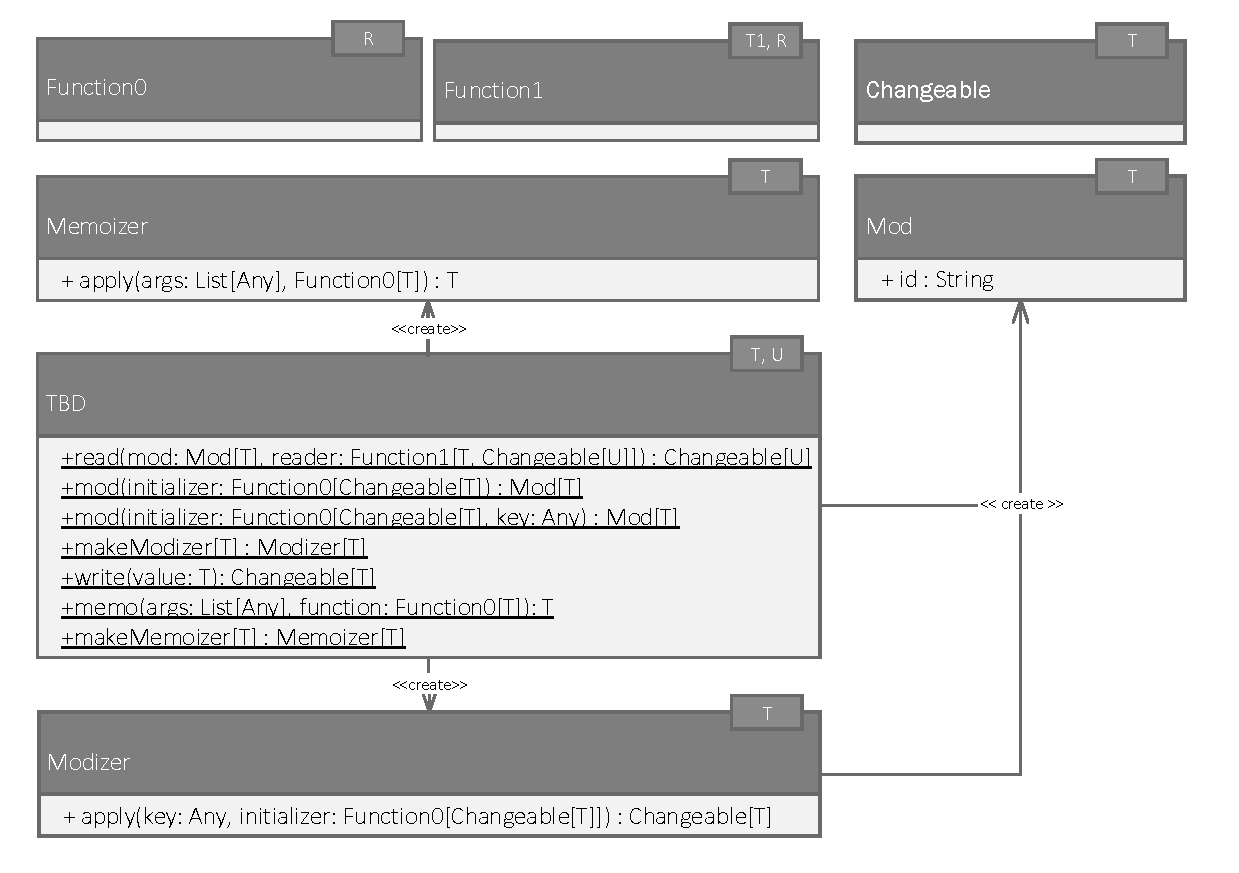
\includegraphics[scale=0.7]{uml/TBD.pdf}
\end{center}
\caption{An UML class diagram for some parts of the TBD API}
\label{fig:tbd_uml}
\end{figure}

Mods are allocated by calling the $mod$ function. The $mod$ function requires a closure without any parameters as first argument. The code contained in this closure is responsible for writing to the allocated memory location exactly once, by issuing a $write$ call. The write call must be the last operatione executed within the closure. Additionally, there is an overload of the $mod$ function, which accepts a key of any type as second parameter. This key is used to provide keyed allocation, as described in section \ref{sec:keyed_alloc}. 

Using the same key in different parts of the programm would break keyed allocation, since the program would overwrite memory which is allocated by another part of the programm. This can happen, for example, if an input list is passed to two different functions and the list elements themselves are used as keys. Therefore, it is possible to create a so called $Modizer$, an object which provides the same functionality as the $mod$ function, but only matches a key if the $Modizer$ instance is also the same. This means that a $Modizer$ can be used to provide keyed allocation independently from other parts of the program. 

To read a mod, the $read$ function has to be used. The $read$ function requires a modifiable as first parameter, and a closure as second paramter. The closure has to take a single parameter, the value of the mod which has been read. The value of the mod is only valid within the closure. When the value of the modifiable changes, the closure is re-executed with the new value during change propagation. 

The $write$ operation takes a single parameter, the value to write to a previously allocated modifiable. The last operation in each closure passed to a $read$ or $mod$ call has to be a $write$ operation. This is enforced by requireing a return type of $Changeable[T]$ from the closure. Objects of type $Changeable[T]$ can only be instantiated by the $write$ call. 

TBD uses explizit memoization. This is done using a $memo$ operation. The first argument of the $memo$ operation is a list of objects which represent the state of the function to call. If this list equals for two calls, a memo match occours. The second parameter is the closure to memoize. As with $mod$, the $memo$ operation also supports independent memoization for certain parts of the application by creating an instance of the class $Memoizer$.

%Parallelism is also supported. The $par$ operator accepts two closures as arguments, which have to return a modifiable and are executed in parallel. This feature of TBD is not of importance for this writing.

It should be noted that each of the described calls requires another argument of the type $Context$, which holds information internally necassary for the operation of TBD. This argument is, however, marked as implicit. This means that the scala compiler automatically passes an available instance of $Context$ to the function, so the programmer does not have to worry about it.  

Also, TBD supports parallel execution and a range of helper methods, which are not outlined here. 

\subsection{Programming patterns for TBD}

As mentioned before, TBD enforces that the last call in each closure passed to $read$ or $mod$ has to be a $write$ call. This means that calls are usually nested, with a $mod$ call at the top, one or more $read$ calls beneath, and a $write$ call at the bottom. Since a program might use more complex data structures, new modifiables may also be created inside the $read$ calls. However, those modifiables must be contained in the final result in some form. Depending on the architecture of the program, it might be possible to add a $memo$ call before a $mod$ call for memoization. Also, the closure-driven programming model does not support loops. Therefore TBD programs are usually recursive. 

Figure \ref{code:add_example} shows the implementation of a basic function, which takes two numbers, adds them, and returns the result as modifiable. 

The first line is a function declaration in Scala. The function's name is $add$. The parameter list is located in the second line. The function accepts two parameters $aMod$ and $bMod$, both of type $Mod[Int]$ and returns a $Mod[Int]$. $Mod[Int]$ is a modifiable holding an integer. In the third line, an additional parameter list is shown. The context parameter in this parameter list is marked as implicit and will automatically be set by the compiler, when calling the $add$ function. Since the calls to $read$, $write$, $memo$ and $mod$ need an instance of context, we have to declare it here. 

The fourth line is responsible for memoization. In this case we check for memo matches using the input variables, $aMod$ and $bMod$. Note that we are able to pass a code block as closure to the function. This is a feature of the Scala language. Whenever no memo match occours, the $memo$ operation will call the passed closure. 

The fifth line allocates a new modifiable using the $mod$ function. In line six, we read the first argument, $aMod$. 

In the seventh line, the read value is bound to a local variable using a $case$ statement from the Scala pattern matching engine. The reason we have to use pattern matching here is that it is impossible to introduce a variable without declaring it. Note that it would not have been sufficient to simply declare a local variable here, since TBD has to assign the variable a value from the outside of the Closure. The local variable $a$ is automatically inferred to be of type $Int$ by the compiler, the symbol $=>$ originates from the Scala syntax for $case$ statements. Also, we issue a read call, which reads the second parameter, $bMod$.

In the eight line, the read value of the second parameter is bound to the local variable $b$. A $write$ call which writes $a + b$ to the allocated mod is issued. The $write$ call automatically places the value in the last allocated modifiable. 

When executing this program, each function executes the passed closure before returning. This means that the $mod$ call returns not until the $write$ operation has finished. 

\begin{figure}
\begin{lstlisting}[frame=single,basicstyle=\ttfamily,numbers=left]
def add
  (aMod: Mod[Int], bMod: Mod[Int])
  (implicit context: Context): Mod[Int] = {
  memo(aMod, bMod) {
    mod {
      read(aMod) {
        case a => read(bMod) {
          case b => write(a + b)
        }
      }
    }
  }
}

\end{lstlisting}
\caption{A basic example of a function which adds two mods, utilizing $read$, $write$, and $mod$}
\label{code:add_example}
\end{figure}

\section{DDG format for TBD}

Since TBD does not perform memoization and re-evaluation on a function level, but rather by introducing specialized functions, we also introduce a new, more specific DDG format for TBD. Figure \ref{fig:add_ddg} illustrates the DDG of a call to the $add$ function from listing \ref{code:add_example} with the input values one and three. The gray square represents the root node, from which our program is called. The green diamond node represents the memo call, the red circled node the mod node, the blue circled nodes the read nodes, and the orange circled node the write node. The type of each node is explicitely annotated and prepended with the node id. The signature of the function call is shown below the node id and type. 

The input and output of the program are not represented in this figure, data dependencies are also not explicitely marked. These details are intentionally omitted, since for complex functions, those graphs would get very complicated. The control dependencies, however, can clearly be seen. Control edges always go from top to bottom. The labels of each node represent the state of the corresponding call. All variables in the signature of the form $d.\alpha$ refer to mods, where $\alpha$ refers to the id of the modifiable. All variables of the form $f.\beta$ refer to anonymous functions in the sourcecode, where for two variables with equal $\beta$, the same function has been called, although the arguments might have been different. Note that those DDGs are usually generated during execution of the program, and therefore also include specific details, like file and line number of the called function. However, this information is not necessary through this writing and therefore not included. 

\begin{figure}
\centering
\begin{tikzpicture}[font=\sffamily,very thick,level/.style={sibling distance=30mm}]
\tikzstyle{every node}=[font=\small]
\node [root, label={0:1.root}]{}
child {
  node [memo, label={0:2.memo}, label={350:(d.1, d.2, f.0)}]{}
  child {
    node [mod, label={0:3.mod}, label={350:(d.3, f.1)}]{}
    child {
      node [read, label={0:4.read}, label={350:(d.1, 1, f.2)}]{}
      child {
        node [read, label={0:5.read}, label={350:(d.2, 2, f.3)}]{}
        child {
          node [write, label={0:6.write}, label={350:(3, d.3)}]{}
        }
      }
    }
  }
};
\end{tikzpicture}
\caption{DDG of the simple $add$ function}
\label{fig:add_ddg}
\end{figure}

In our example, it can be seen that the $memo$ call memoized two modifiables, with the ids $d.1$ and $d.2$. Those modifiables are our input mods. Then, the $memo$ call invoked an anonymous function $f.0$. The function $f.0$ refers to the function starting at line two in our example, in which a $mod$ call was executed. The $mod$ call then allocated a new modifiable with id $d.3$ and called the anonymous function $f.1$, starting in line three in our example. Inside this function, $d.1$ with value $1$ and $d.2$ with value $2$ were read by two consecutive $read$ calls. Finally, the innermost anonymous function, $f.3$, which refers to the function starting in line four, is executed. Inside this function call, the result, three, is written to the allocated modifiable $d.3$. 

When observing the ids of the modifiables in $read$, $mod$ and $write$ executions closely, dependencies can be found. In this case, we have an allocate-write dependency between the $mod$ and the $write$ instruction, since we allocate the mod $d.3$ and then write to it. Also, it should be noted that the innermost function $f.3$ closes over the the variable $a$ introduced by the first $read$ instruction, and therefore binds it. This detail is of importance later. 

\section{The Map Operator implemented on Top of TBD}

To wrap up this section, we revisit the map example introduced in section \ref{sec:simple_example} and theoretically discussed in section \ref{sec:ddg}. Since the map operator operates on lists, we define a list element class, $SimpleList$, which is shown in \ref{fig:simple_list_uml}. The $SimpleList$ class represents a single item. Each instance has a member which points to the next element of the list, and a member which holds the value. The head of a list is represented by an instance of $Mod[SimpleListElement[T]]$, the last element in the list is represented by a modifiable which holds a null reference.  

\begin{figure}
\begin{center}
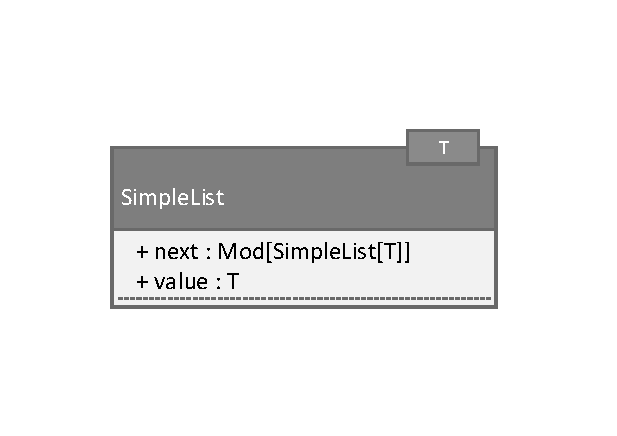
\includegraphics[scale=0.7]{uml/SimpleList.pdf}
\end{center}
\caption{An UML class diagram for a simple linked list}
\label{fig:simple_list_uml}
\end{figure}

Since the list head and each next element are represented as modifiables, we introduce a wrapper class which adds a map method to instances of $Mod[SimpleListElement[T]]$, and mark it as implicit. This way, the scala compiler automatically wraps all instances of $Mod[SimpleListElement[T]]$ where applicable. 

In our wrapper class, we define the method map. The implementation can be seen in Listing \ref{code:map_example}. As arguments we supply a function parameter, $mapper$, which maps the value of each element of type $T$ to a new value of type $U$, and an instance of the $Memoizer$ class. 

In line six we memoize against the $Mod[SimpleList[T]]$ instance $currentElement$, which reprents the list element we are operating on. Then, we create a new modifiable for the new element in line seven and read the current element in line eight. If the current element is null, we reached the end of the list, and we write the final element of our output list in line nine. If the current element is not null, we write a new list element in line ten. The value of the new list element is the result of the call to the $mapper$ function. The next element of the new element is the result of a recursive application of the $map$ function to the successor of this element. 

\begin{figure}
\begin{lstlisting}[frame=single,basicstyle=\ttfamily,numbers=left]
def map[U]
  (mapper: T => U, 
  memoizer: Memoizer[Mod[SimpleList[U]]])
  (implicit c: Context):
    Mod[SimpleList[U]] = {
  memoizer(currentElem) {
    mod {
      read(currentElem) {
        case null => write(null)
        case elem => write({
          val newValue = mapper(elem.value)
          val newNext = elem.next.map(mapper, memo)
          new SimpleList(newValue, newNext)
        })
      }
    }
  }
}
\end{lstlisting}
\caption{A map function implemented on top of TBD}
\label{code:map_example}
\end{figure}

%generated using: 
%bin/visualization.sh -a smmap -t manual -i 1  
%u 1 0
%a 2 1
%a 3 2
%a 4 3
%p

\begin{figure}
\centering
\begin{tikzpicture}[font=\sffamily,very thick,level/.style={sibling distance=40mm}]
\tikzstyle{every node}=[font=\small]
\node [root, label={0:1.root}, label={350:}]{}
child {
  node (2)[memo, label={0:2.memo}, label={350:(f.23, 1, Mod(d.0))}]{}
  child {
    node (3)[mod, label={0:3.mod}, label={350:(d.2, f.22)}]{}
    child {
      node (4)[read, label={0:4.read}, label={350:(d.0, (1,71), f.21)}]{}
      child {
        node (10)[memo, label={0:10.memo}, label={350:(f.23, 1, Mod(d.1))}]{}
        child {
          node (11)[mod, label={0:11.mod}, label={350:(d.7, f.22)}]{}
          child {
            node (12)[read, label={0:12.read}, label={350:(d.1, (2,1), f.21)}]{}
            child {
              node (13)[memo, label={0:13.memo}, label={350:(f.23, 1, Mod(d.4))}]{}
              child {
                node (14)[mod, label={0:14.mod}, label={350:(d.8, f.22)}]{}
                child {
                  node (15)[read, label={0:15.read}, label={350:(d.4, (3,2), f.21)}]{}
                  child {
                    node (16)[memo, label={0:16.memo}, label={350:(f.23, 1, Mod(d.5))}]{}
                    child {
                      node (17)[mod, label={0:17.mod}, label={350:(d.9, f.22)}]{}
                      child {
                        node (18)[read, label={0:18.read}, label={350:(d.5, (4,3), f.21)}]{}
                        child {
                          node (19)[memo, label={0:19.memo}, label={350:(f.23, 1, Mod(d.6))}]{}
                          child {
                            node (20)[mod, label={0:20.mod}, label={350:(d.10, f.22)}]{}
                            child {
                              node (21)[read, label={0:21.read}, label={350:(d.6, null, f.21)}]{}
                              child {
                                node (22)[write, label={0:22.write}, label={350:(d.10, null)}]{}
                              }
                            }
                          }
                        }
                        child {
                          node (23)[write, label={0:23.write}, label={350:(d.9, (4,6))}]{}
                        }
                      }
                    }
                  }
                  child {
                    node (24)[write, label={0:24.write}, label={350:(d.8, (3,4))}]{}
                  }
                }
              }
            }
            child {
              node (25)[write, label={0:25.write}, label={350:(d.7, (2,2))}]{}
            }
          }
        }
      }
      child {
        node (26)[write, label={0:26.write}, label={350:(d.2, (1,0))}]{}
      }
    }
  }
};
\begin{pgfonlayer}{background}
\fill[blue,opacity=0.2] \convexpath{2,26,4,3}{8pt};
\fill[blue,opacity=0.2] \convexpath{10,25,12,11}{8pt};
\fill[blue,opacity=0.2] \convexpath{13,24,15,14}{8pt};
\fill[blue,opacity=0.2] \convexpath{16,23,18,17}{8pt};
\fill[blue,opacity=0.2] \convexpath{19,22,21,20}{8pt};
\end{pgfonlayer}
\end{tikzpicture}
\caption{DDG of the $map$ function with input $(0, 1, 2, 3)$.}
\label{fig:map_tbd_ddg}
\end{figure}


Figure \ref{fig:map_tbd_ddg} shows the DDG of a call of the map function with the input list $(0, 1, 2, 3)$. Regarding the basic structure, the DDG is identical to the DDG in figure \ref{fig:map_ddg}. The node sets $\{2, 3, 4, 26\}$, $\{10, 11, 12, 25\}$, $\{13, 14, 15, 24\}$ and $\{15, 17, 18, 23\}$ correspond to a single call of the map function from figure \ref{fig:map_ddg} each. The nodes $\{19, 20, 21, 22\}$ represent writing the end of the list. Each of those sets also corresponds to a single recursive call of the map function described in listing \ref{code:map_example}, where each $memo$ node corresponds to the $memo$ call in line six, each $mod$ node to the $mod$ call in line seven, each $read$ node to the $read$ call in line eight and each $write$ node except the last to the write call in line ten. The last $write$ node corresponds the $write(null)$ call in line nine. Those groupes which correspond to a single recursive call of the $map$ function can be identified by consulting the function ids inside the signatures. For instance, the memo node at the beginning of each call invokes the closure $f.23$. 

\chapter{Calculating Trace Distance}
\label{ch:implementation}

Consulting DDGs can greately ease the debugging of TBD programs. Not only bugs in algorithms can be found quicker, also the prerformance of the program can be analysed. When we update the input and run change propagation for any program, the program state updates and therefore the DDG changes. By comparing the DDGs of two exectutions of the same program with two different inputs each, we can inspect how well the program handled change propagation. It is feasiable to assume that each closure in a TBD program can be executed in constant time, excluding subcalls to $mod$, $read$ or $memo$ the closure containes. The reason is that control structures like loops are not available in TBD programs. Iterating over input elements has to be done using recursion, where each recursion step places new $read$ calls. It should be noted that it is possible to write programs which do not satisfy this condition, for example by putting the whole input into an array stored in a single mod, reading that mod and iterating over the whole array at once. Such a program would, however, perform really bad when propagating input changes and miss the point of incremental computation.  

We call the difference between to DDGs of two different executions of the same program \textit{Trace Distance}. This name originates from the fact that all nodes and control edges of a DDG resemble a program executiont race. As already mentioned, calculating trace distance is straight forward using a greedy matching. We create two sets $A$ and $B$, where $A$ holds all nodes of the first DDG and $B$ holds all nodes of the second DDG. Foreach node in $A$, we search $B$ for an equivalent node. If we find an equivalent node, we remove both nodes from $A$ and $B$, respectively. The count of remeaning nodes, or formally $|A| + |B|$ is the trace distance of the two DDGs. 

The interesting part here, however, is how we define equality of nodes. In this chapter, we explain how it is possible to create multiple, meaningful definitions of equality, which result in different meaningful results for trace distance. 
  
\section{Node Tags}
For checking node equality, we create so called \textit{Node Tags}. A node tag is a ordered sets of values associated with a single node. When checking nodes for equality, we simply check whether the node tags equal. To ease the definition of node tags, we introduce a \textit{Function Tag}, which can be used inside node tags. The function tag uniquely represents a closure by holding an unique function id and the name and value of all free variables bound from by the closure from an outer scope. If two function tags are equal, the corresponding closures are also equal. 

Since closures can also contain values which are read or written in the program, it is important that all data structures used by the program implement a meaningful method to check for equality. Modifiables form an exception and can be compared by comparing the id of the modifiable, regardless of the stored value. 

[Todo: \"Full\" trace distance, \"Program-Only\" trace distance, \"Allocation-Insensitivie\" trace distance: Describe and find more suitable names.]

%\chapter{Implementation}
%\label{ch:impl}
%The main problem is that DDG nodes, which represent function calls, have to be compared for equality. The problem of comparing functions in general is, however, one of the unsolved problems of computer science. 

%\section{Architecture}

%\section{Data Collection}

%\subsection{Usage of Scala Macros}

%\chapter{Use Cases}
%\label{ch:use_cases}

%\chapter{Discussion}
%\label{ch:discussion}